\chapter{Case Study}
\thispagestyle{plain}

\section{Instance description}
In this chapter, we present a case study of a well known scheduling instance from \cite{KONDILI1993211}, optimized for the deterministic case using the described online tool. The production of two products 1 and 2 from three feed stocks A, B and C takes place according to the STN representation given in Fig. \ref{fig:STN}. This instance has four intermediate states and five tasks.

\begin{figure}[htb]
\centering
\fbox{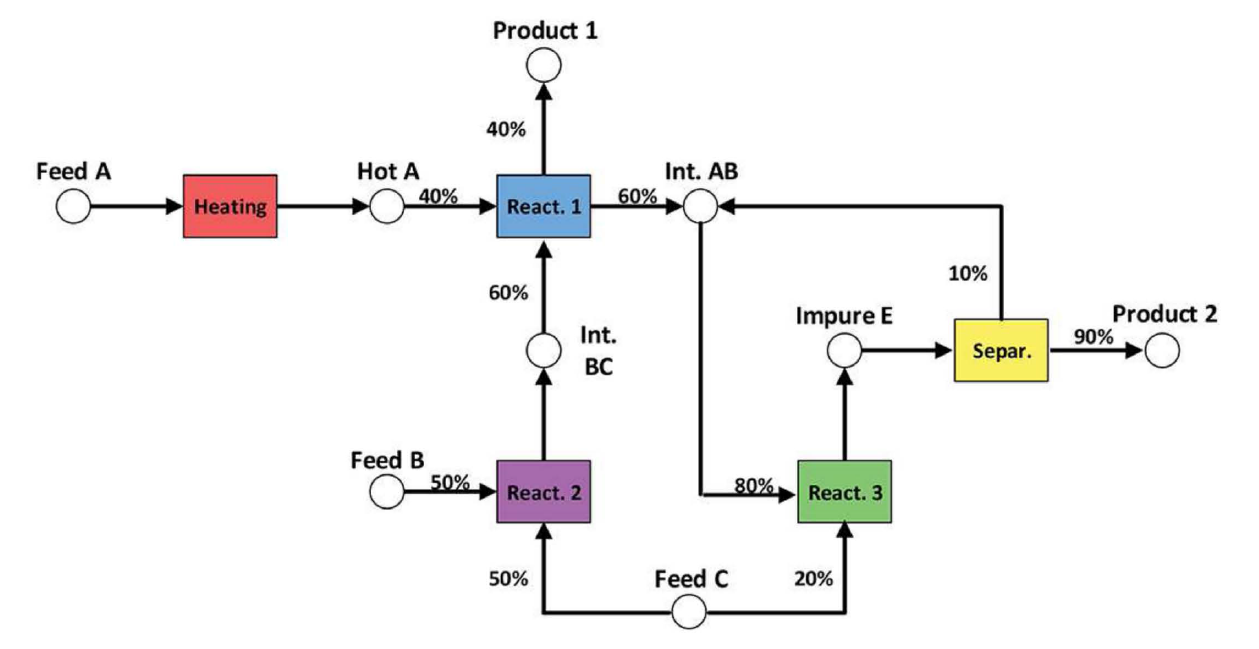
\includegraphics[width=\linewidth]{Images/STN.png}}
\caption{State task network for the example instance}
\label{fig:STN}
\end{figure}

Table \ref{tab:statelevels} shows the state maximum capacity and initial load data for the problem. The available unit, task compatibility and processing time data is given in Table \ref{tab:tasks}.

\begin{table}[htb]
\centering
\caption{Problem data (states)}
\label{tab:statelevels}
\begin{tabular}{@{}cccc@{}}
\toprule
\textbf{State} & \textbf{Capacity} & \textbf{Initial load} & \textbf{Price (per unit)} \\ \midrule
Feed A         & 1000              & 1000                  & -                         \\
Feed B         & 1000              & 1000                  & -                         \\
Feed C         & 1000              & 1000                  & -                         \\
Hot A          & 100               & -                     & -                         \\
Int. BC        & 200               & -                     & -                         \\
Int. AB        & 150               & -                     & -                         \\
Impure E       & 200               & -                     & -                         \\
Product 1      & 1000              & -                     & 10                        \\
Product 2      & 1000              & -                     & 10                        \\ \bottomrule
\end{tabular}
\end{table}

\begin{table}[htb]
\centering
\caption{Problem data (units \& tasks)}
\label{tab:tasks}
\begin{tabular}{@{}ccccccccc@{}}
\toprule
Unit         & \multicolumn{2}{c}{Heater} & \multicolumn{2}{c}{Reactor 1} & \multicolumn{2}{c}{Reactor 2} & \multicolumn{2}{c}{Separator} \\ \cmidrule(l){2-9} 
Maximum Load & \multicolumn{2}{c}{100}    & \multicolumn{2}{c}{50}        & \multicolumn{2}{c}{80}        & \multicolumn{2}{c}{200}       \\ \midrule
Tasks        & $\alpha$       & $\beta$       & $\alpha$         & $\beta$        & $\alpha$         & $\beta$        & $\alpha$         & $\beta$        \\ \cmidrule(l){2-9} 
Heating      & 0.667        & 0.007       &                &              &                &              &                &              \\
Reaction 1   &              &             & 1.334          & 0.027        & 1.334          & 0.017        &                &              \\
Reaction 2   &              &             & 1.334          & 0.027        & 1.334          & 0.017        &                &              \\
Reaction 3   &              &             & 0.667          & 0.013        & 0.667          & 0.008        &                &              \\
Separation   &              &             &                &              &                &              & 1.334          & 0.007        \\ \bottomrule
\end{tabular}
\end{table}

\section{Defining instance parameters}
\subsection{Defining units}
\begin{figure}[htbp]
\centering
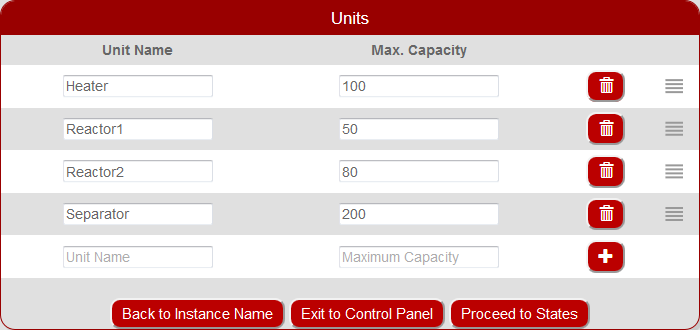
\includegraphics[width=\linewidth]{Images/DefineUnits.png}
\caption{Units input into webtool}
\label{fig:defUnits}
\end{figure}
Unit names and maximum capacities from Table \ref{tab:tasks} are input into the units table of the web tool as shown in Fig. \ref{fig:defUnits}.

\subsection{Defining states}
\begin{figure}[htbp]
\centering
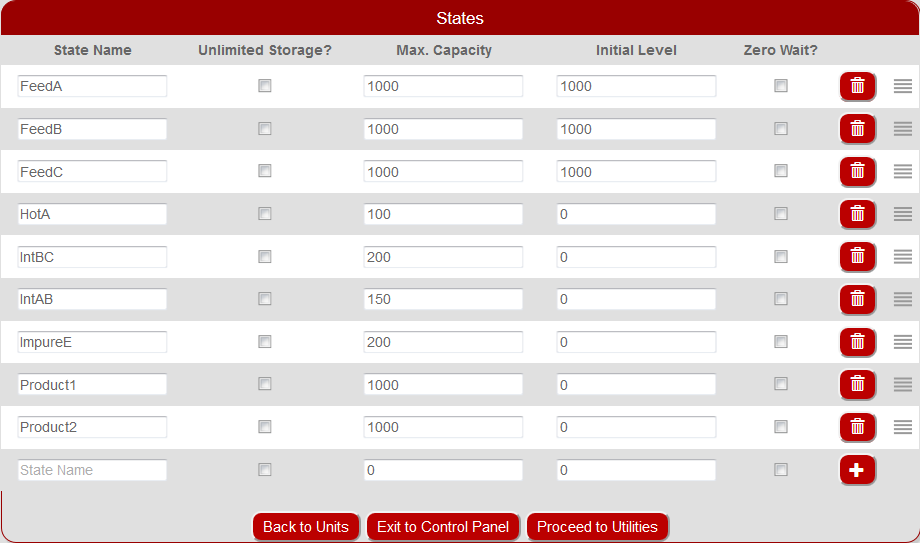
\includegraphics[width=\linewidth]{Images/DefineStates.png}
\caption{States input into webtool}
\label{fig:defStates}
\end{figure}
State names, maximum storage capacities and initial levels from Table \ref{tab:statelevels} are input into the units table of the web tool as shown in Fig. \ref{fig:defStates}.


\subsection{Defining tasks}
\begin{figure}[htbp]
\centering
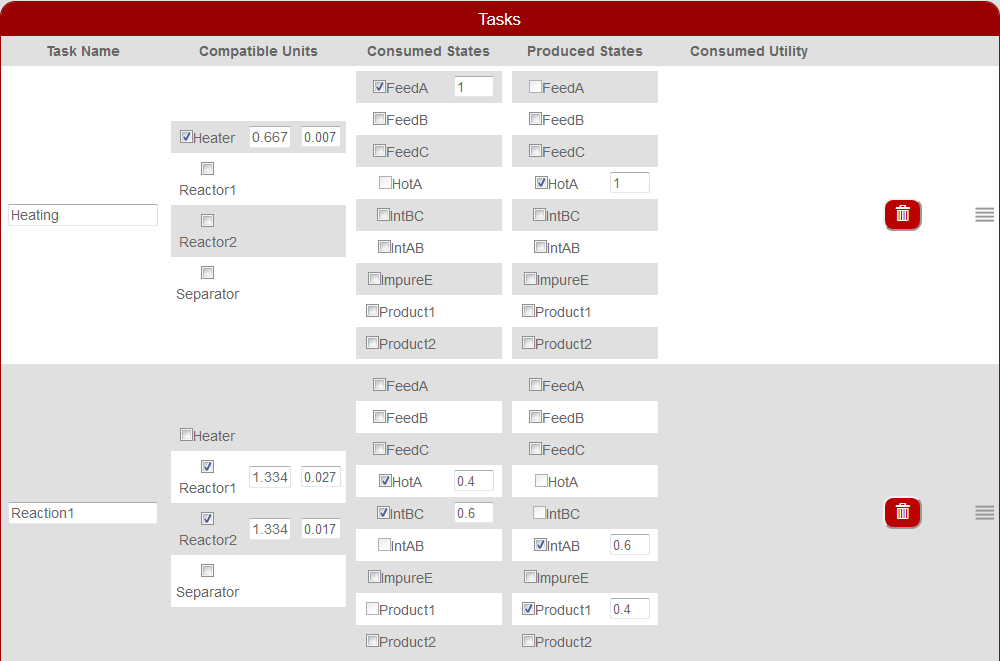
\includegraphics[width=\linewidth]{Images/DefineTasks.png}
\caption{Tasks input into webtool}
\label{fig:defTasks}
\end{figure}

This instance does not involve utilities. Hence we can skip utilities input. For each task in Table \ref{tab:tasks}, the values of $\alpha$ and $\beta$ are input after selecting the appropriate compatible unit(s). Fig. \ref{fig:defTasks} shows the tasks table after successful input of tasks Heating and Reaction 1.


\subsection{Objective}

\begin{figure}[htbp]
\centering

\includegraphics[width=0.8\linewidth]{Images/DefineObjective.png}
\caption{Objective selection}
\label{fig:selectObjective}
\end{figure}

For this case, we will consider the case of maximization of profit. After successful completion of the tasks input, the objective selection options are available as shown in Fig. \ref{fig:selectObjective}. After clicking on ``Maximize profit'', the horizon and price input screen appears as shown in Fig. \ref{fig:prices}. The instance definition is complete after input of horizon and price data for Product 1 and Product 2 from Table \ref{tab:statelevels}. We will consider an 8 hour horizon for this case study.

\begin{figure}[htbp]
\centering
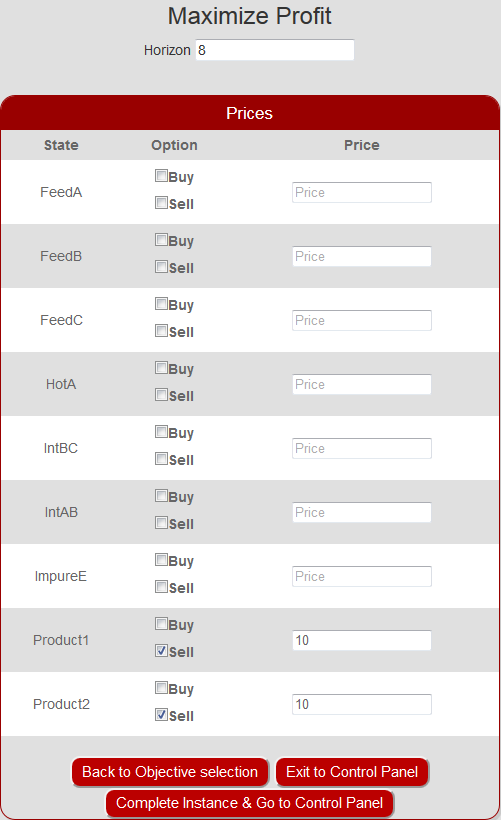
\includegraphics[width=0.8\linewidth]{Images/Prices.png}
\caption{Horizon and price input}
\label{fig:prices}
\end{figure}

\section{Submission}

\begin{figure}[htbp]
\centering
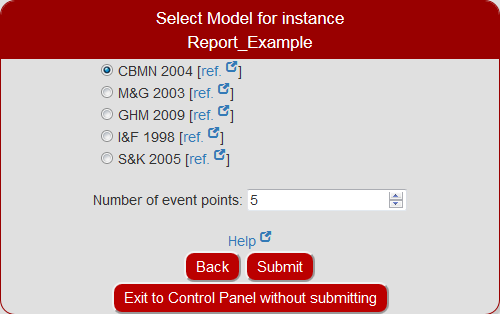
\includegraphics[width=0.8\linewidth]{Images/SelectModel.png}
\caption{Number of event points and model selection}
\label{fig:selectModel}
\end{figure}

Once the instance is complete, the submit button in the control panel will be activated. Clicking the ``Submit'' button will display the model selection table as shown in Fig. \ref{fig:selectModel}. For the deterministic version, the five models described in Chapter \ref{chap:models} are available. The CBMN 2004 model is selected by default. 

\subsection{Number of event points}
\label{subsec:eventpoints}
Continuous-time formulations for short-term scheduling are based on a set of time points (unit specific or global), which are non-uniformly distributed along the scheduling horizon. A limitation of these approaches is that the number of time points required to represent the optimal schedule is unknown a priori, so multiple MILP models need to be solved to reach the optimal solution. A suitable strategy is to start by adopting a small number of event points and gradually increase this number and repeatedly solve the model until the objective values does not show an improvement. For this particular instance, 5 event points result in the optimal schedule. Clicking the ``Submit'' on this page will add the instance to the processing queue.

\section{Results}
\begin{figure}[htbp]
\centering
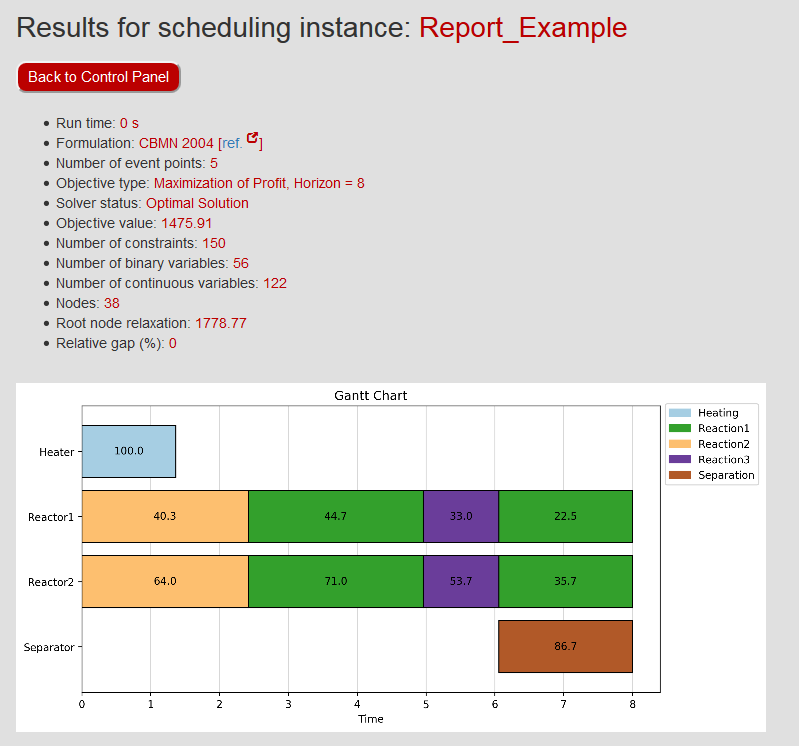
\includegraphics[width=\linewidth]{Images/Results.png}
\caption{Model statistics and Gantt chart}
\label{fig:results}
\end{figure}

Once the processing of the instance has completed, the ``Submission Status'' field on the control panel for the instance will change to ``Results Available''. Clicking on the ``Results'' button will show model statistics and the optimized Gantt Chart as shown in Fig. \ref{fig:results}.

%\begin{figure}[htbp]
%\centering
%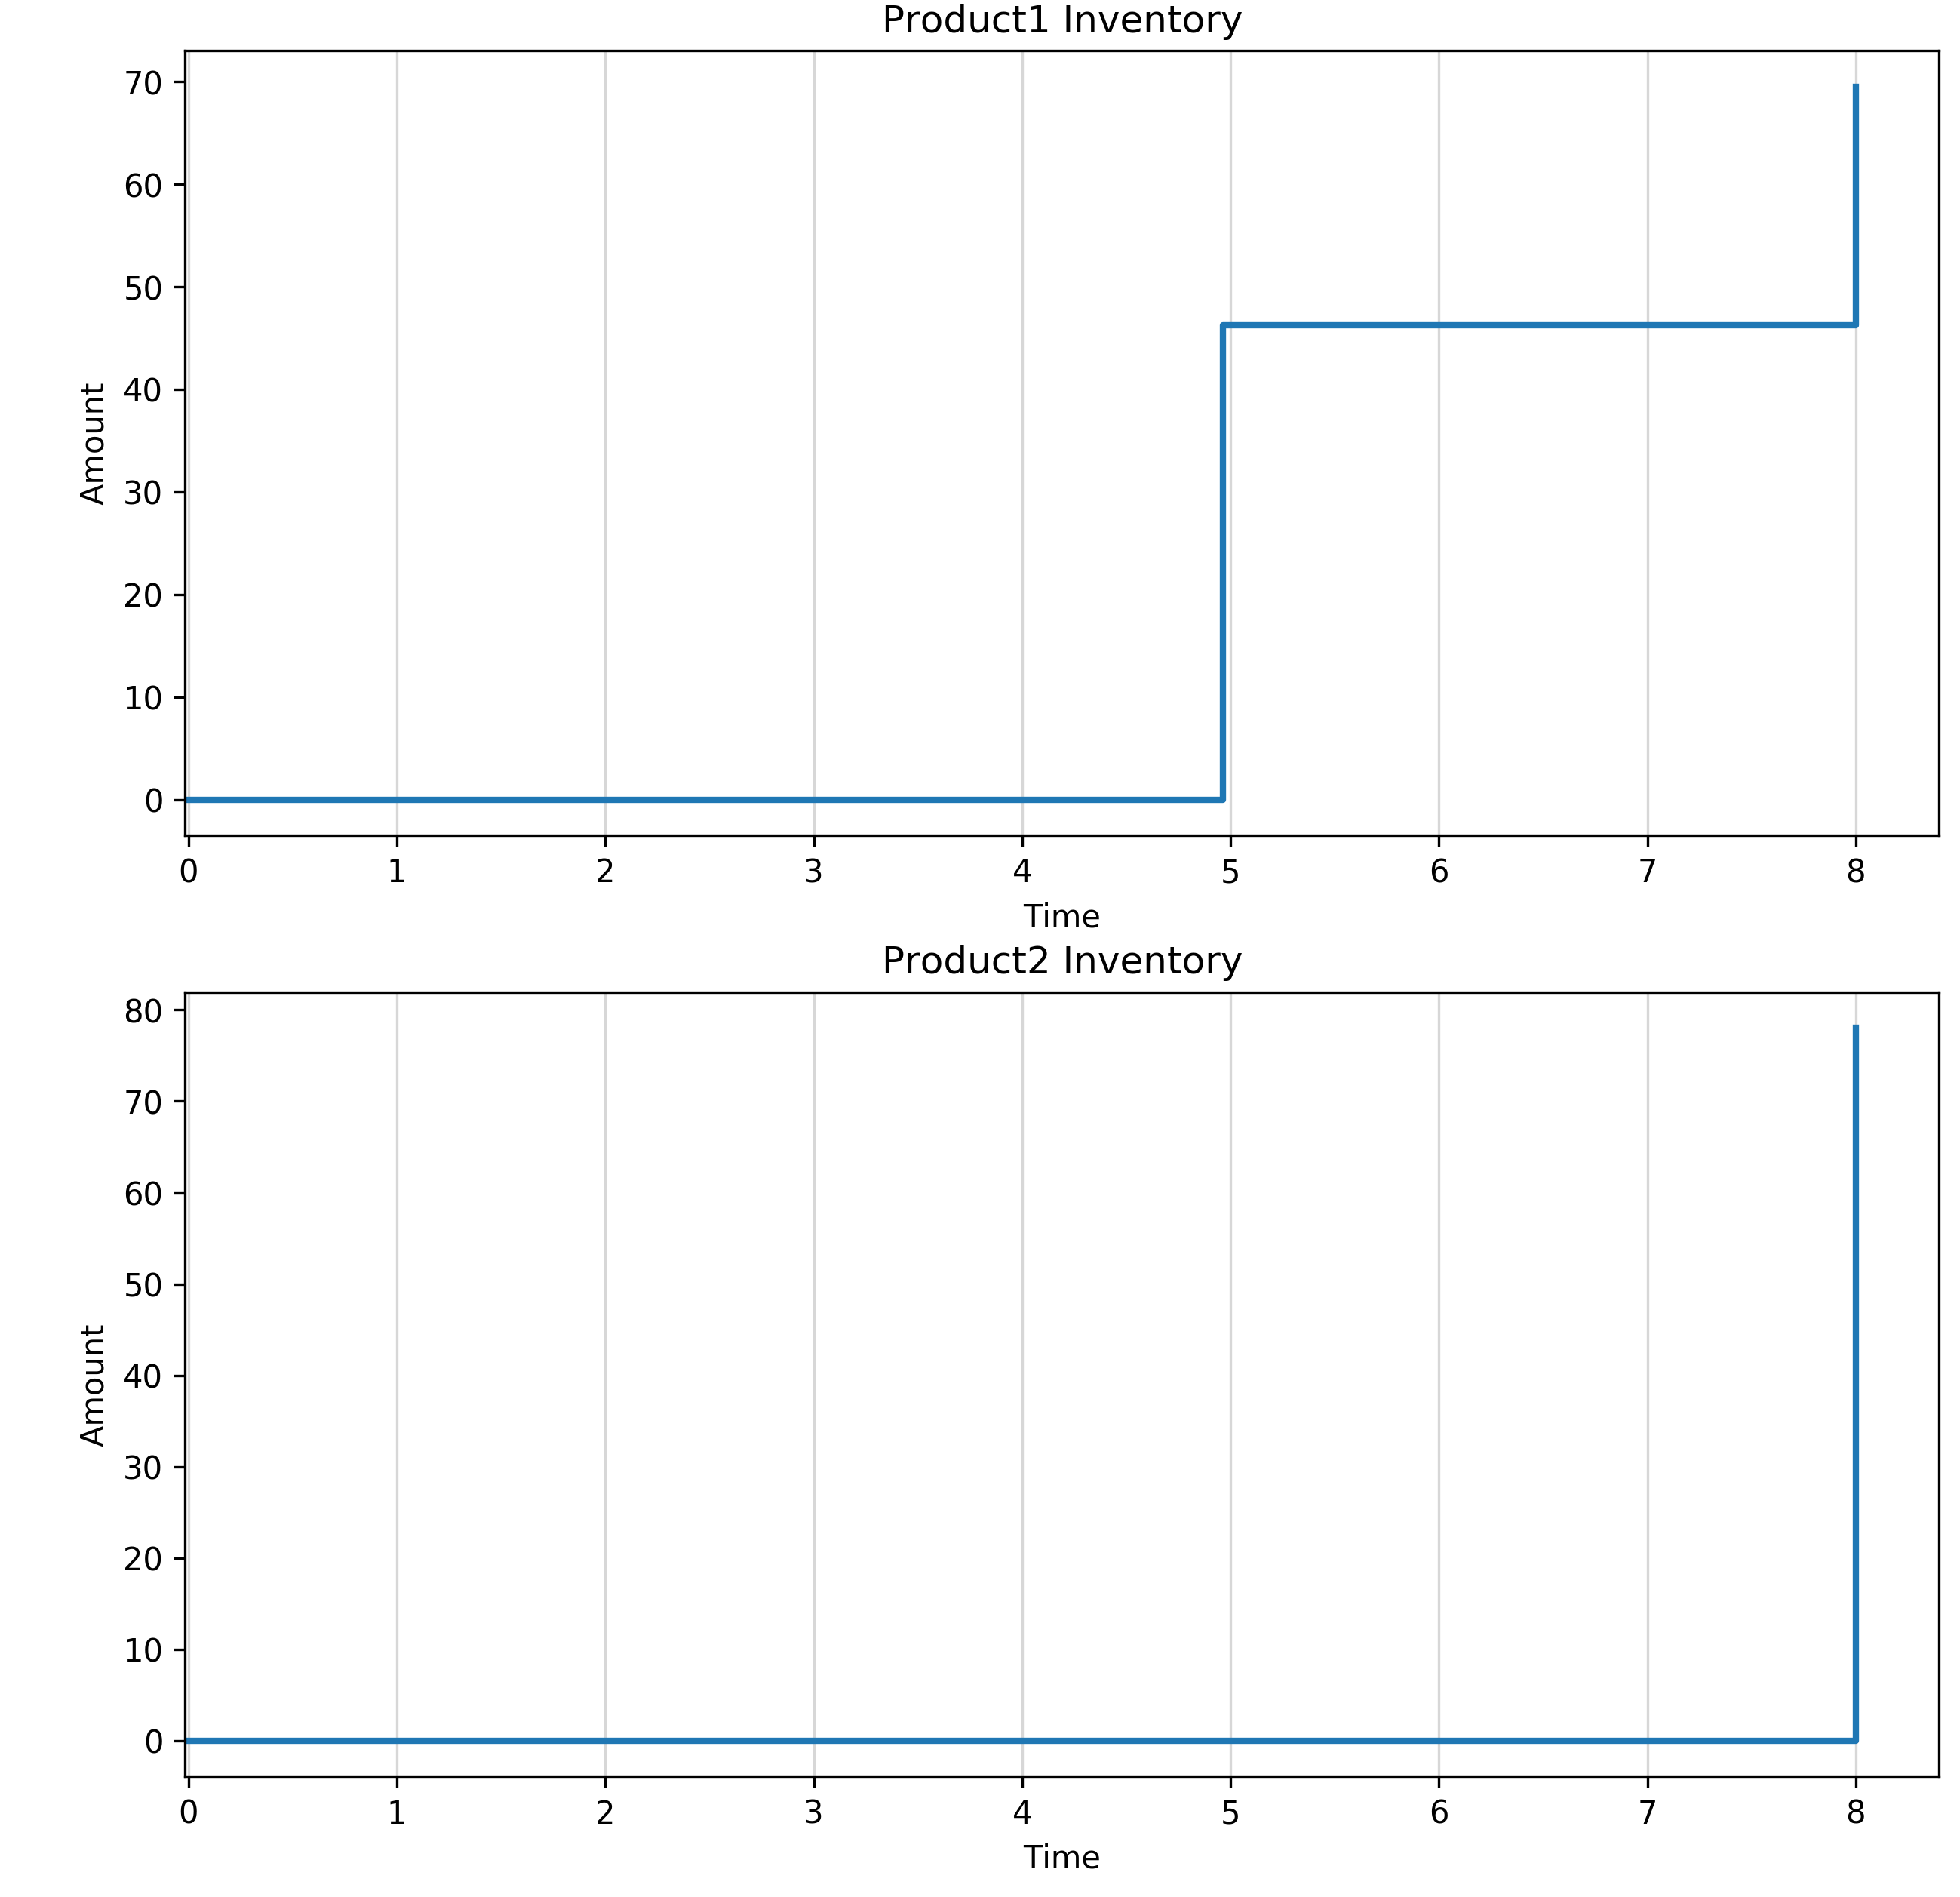
\includegraphics[width=\linewidth]{Images/ProductInventory.png}
%\caption{Product 1 \& Product 2 inventory vs. time}
%\label{fig:stateInventory}
%\end{figure}

A proven optimal solution is found fairly quickly by CPLEX. The objective value reported by the tool is the same as that reported in previous literature for this instance. Inventory level charts for Product 1 and Product 2 show that around 70 units of Product 1 and 80 units of Product 2 will be manufactured.

\section{Handling uncertain parameters with robust optimization}
In this section, we will consider uncertainty in fixed processing time ($\alpha$). The parameters are allowed to vary in a decision-dependent polyhedron. The original $\alpha_i$ values specified by the user are regarded as nominal values $\alpha_i^0$. The maximum allowable magnitude of each parameter's deviation from its nominal value is a percentage of the latter (e.g. $\pm$ 10\% of its nominal value).

In addition, we also consider one general affine correlation to postulate an upper limit on the cumulative processing time deviation among all tasks to be performed. The quantities $\xi \in [0,1]$ and $\phi \in [0,1]$ are used to parameterize the uncertainty set. For low, medium and high uncertainty levels, the values of $\xi$ and $\phi$ are set as follows:
\begin{enumerate}
\item \textbf{Low:} $\xi = 0.1$ , $\phi = 0.0$
\item \textbf{Medium:} $\xi = 0.2$ , $\phi = 0.5$
\item \textbf{High:} $\xi = 0.3$ , $\phi = 1.0$
\end{enumerate}

For the case of static robust optimization, a ``worst-case'' maximum profit objective value of 1312.45 is obtained. For adjustable robust optimization, the corresponding value is 1355.68. Although both of these solutions are worse than the deterministic case, ARO provides an improved solution as compared to SRO. In this case, we have considered a ``Low'' uncertainty level. For the ARO case, timing, batch size and state level variables were considered to be adjustable. The nominal realization Gantt charts are shown in Fig. \ref{fig:GanttSRO} and \ref{fig:GanttARO}. The number of event points for each case was determined using the procedure described in \ref{subsec:eventpoints}. 


\begin{figure}[htb]
  \centering
  \begin{minipage}[b]{0.49\textwidth}
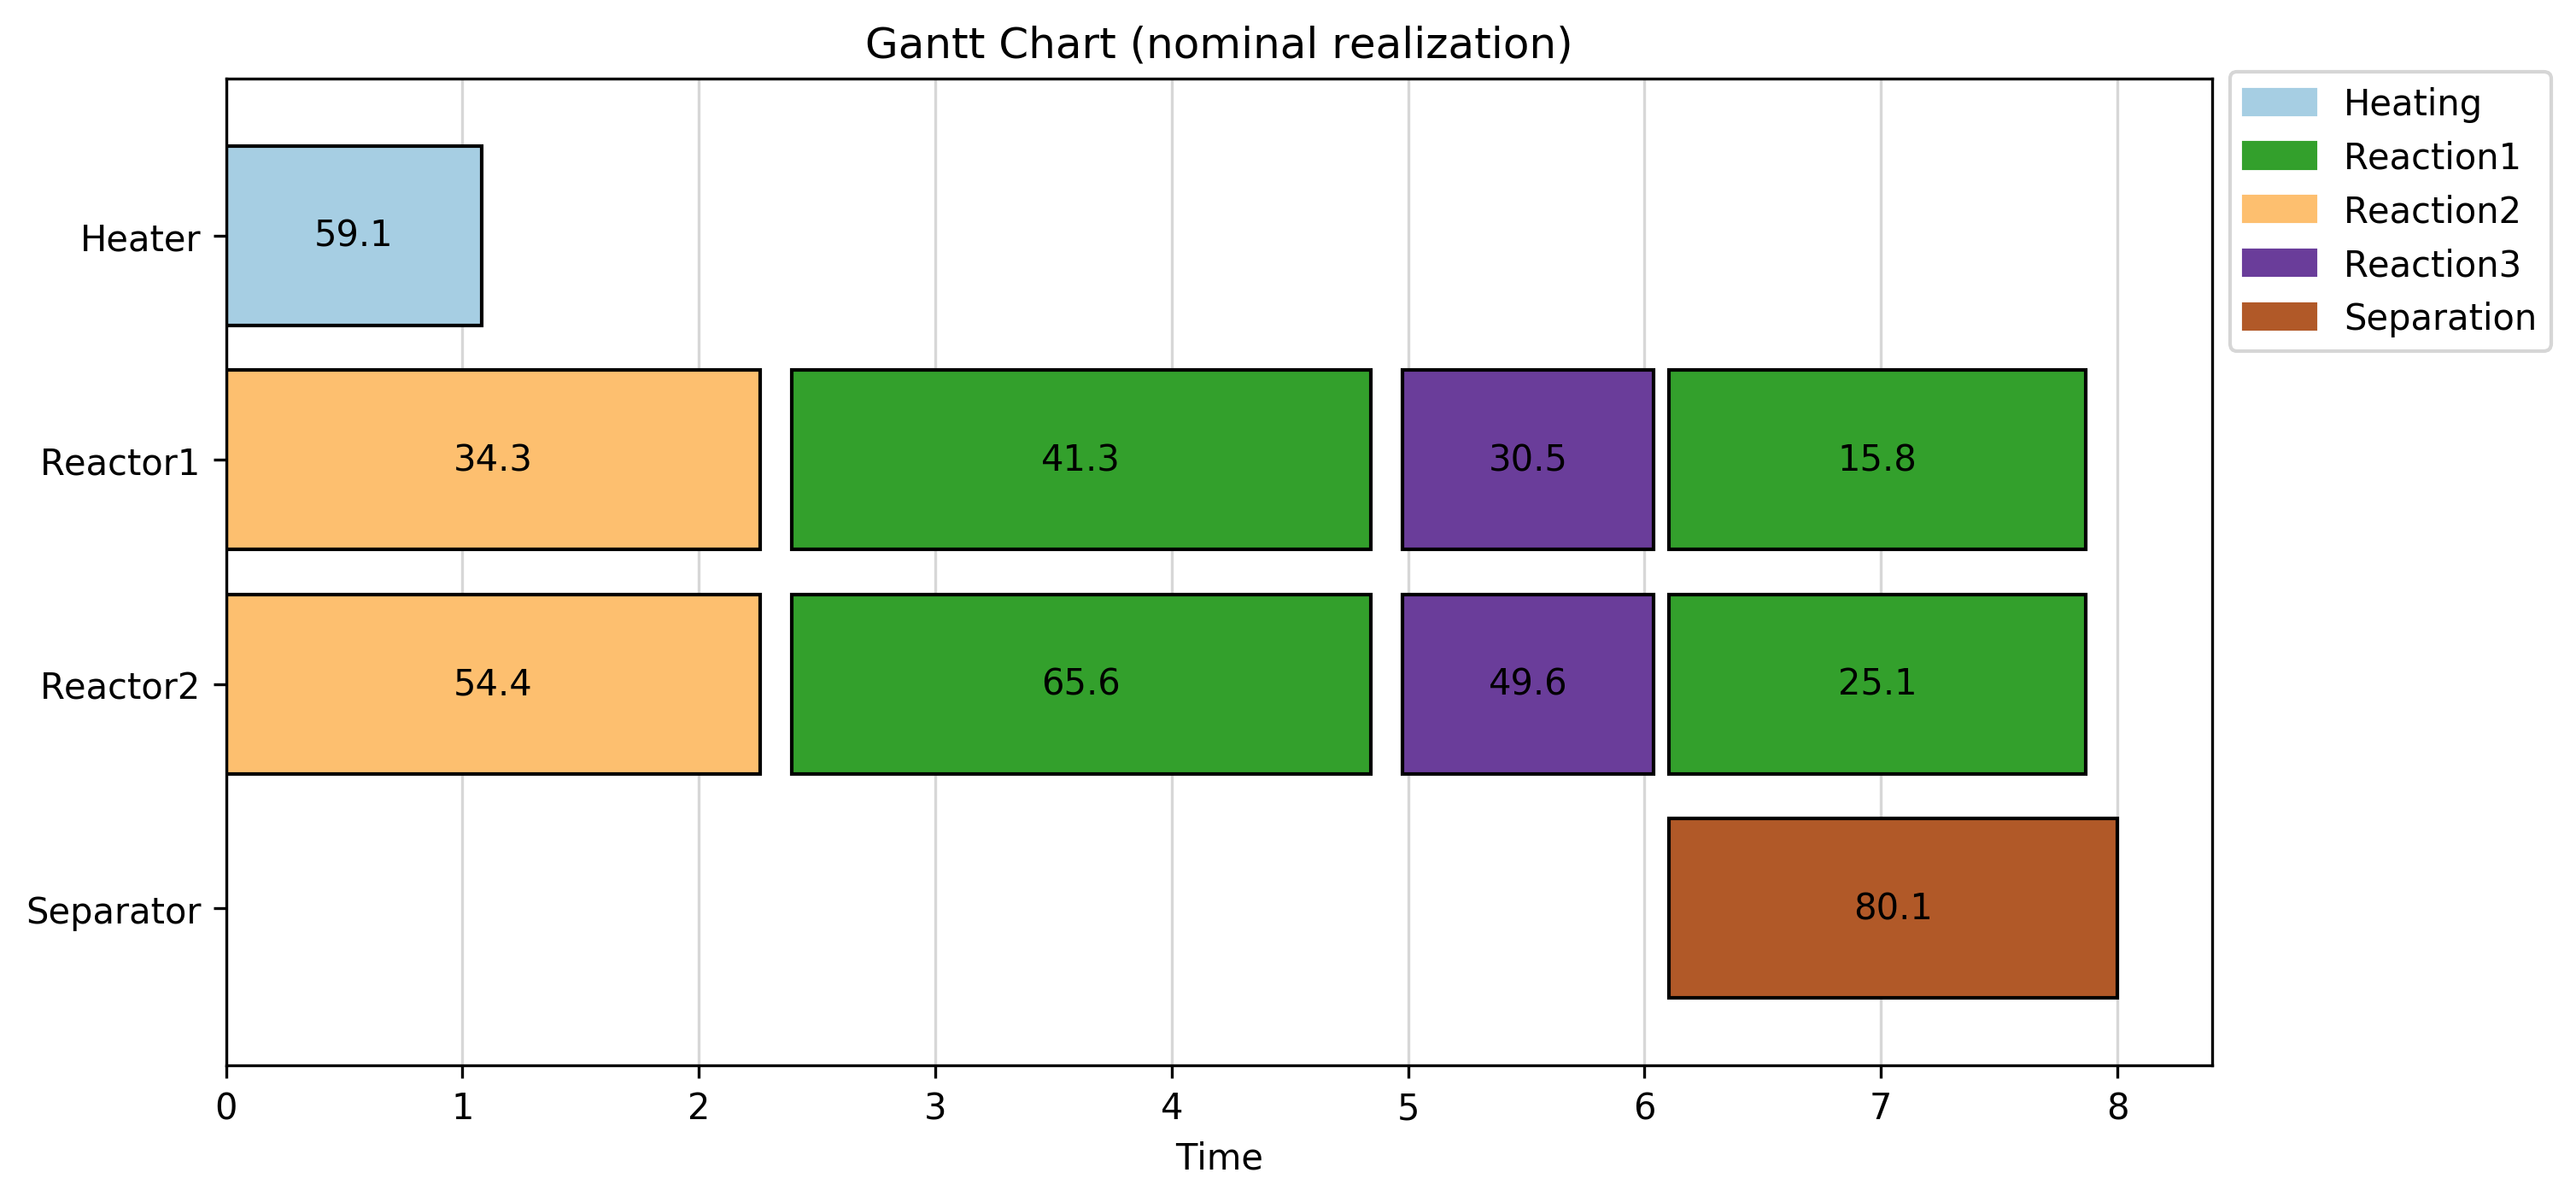
\includegraphics[width=\textwidth]{Images/SRO_Gantt.png}
    \caption{SRO for low uncertainty in fixed processing time (n = 5)}
\label{fig:GanttSRO}
  \end{minipage}
\hfill
  \begin{minipage}[b]{0.49\textwidth}
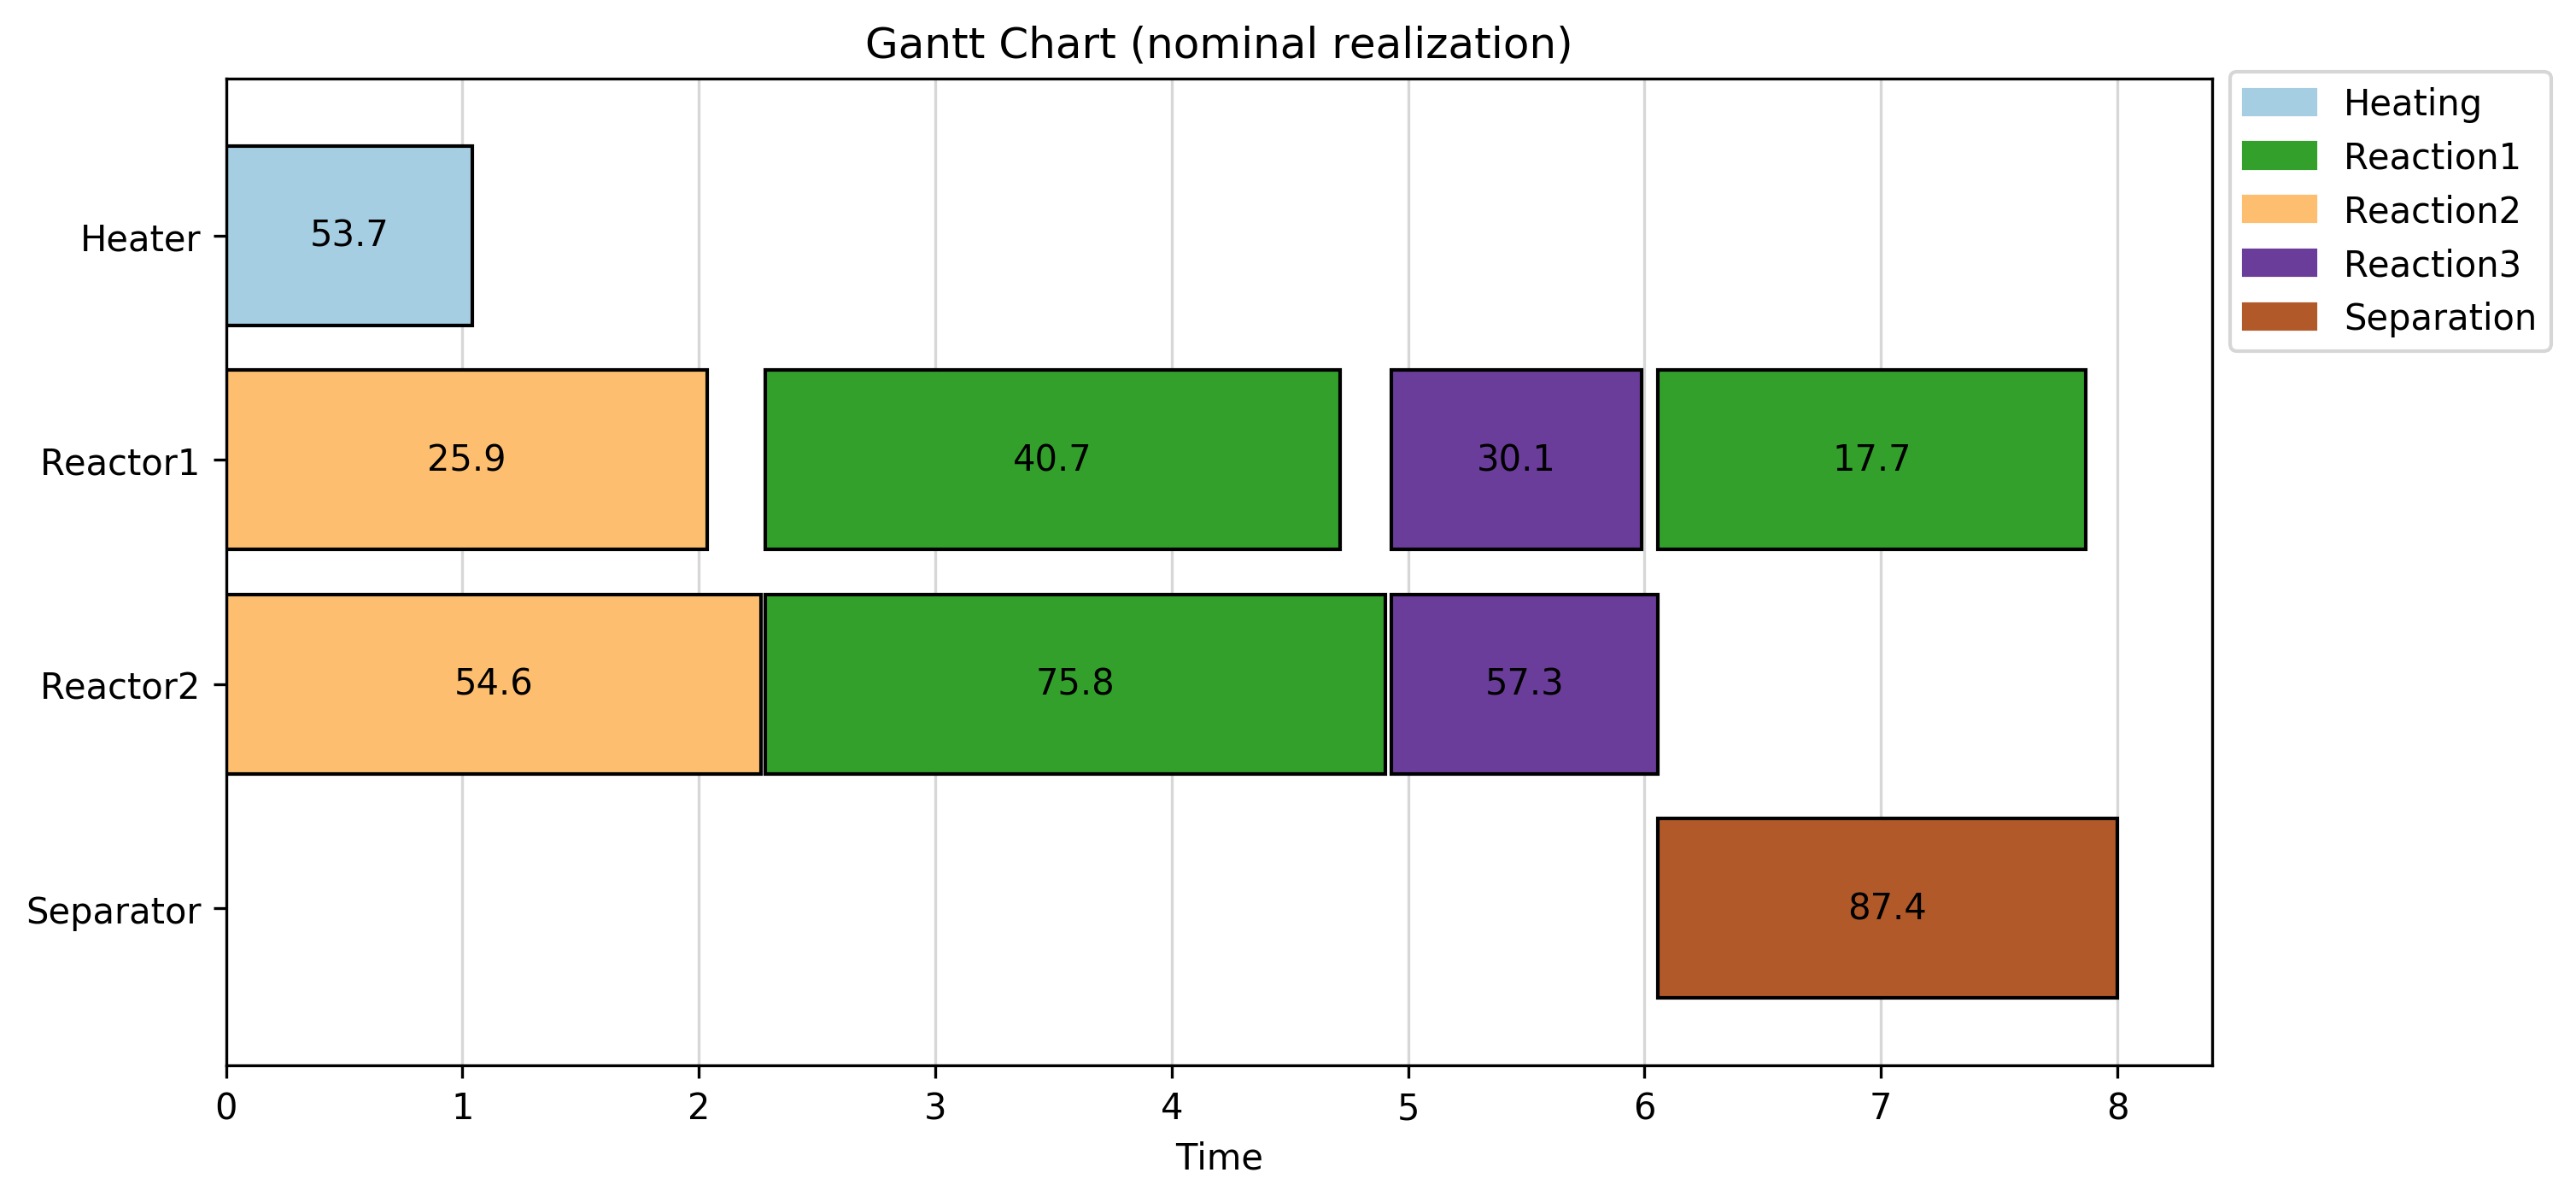
\includegraphics[width=\textwidth]{Images/ARO_Gantt.png}
    \caption{ARO for low uncertainty in fixed processing time (n = 6)}
    \label{fig:GanttARO}
  \end{minipage}
\end{figure}


It is seen that both the robust optimization models are significantly larger than the deterministic models (Table \ref{tab:modelsize}), consequently, they are harder to solve. The ARO problem can only be solved to 0.14\% optimality gap within the one hour time limit. For both these cases, the CBMN 2004 model was used.

\begin{table}[htb]
\centering
\caption{Model size comparision}
\label{tab:modelsize}
\begin{tabular}{@{}lccc@{}}
\toprule
                            & \textbf{Deterministic} & \textbf{SRO} & \textbf{ARO} \\ \midrule
No. of constraints          & 150                    & 4,670         & 118,579       \\
No. of binary variables     & 56                     & 96           & 144          \\
No. of continuous variables & 122                    & 9,194         & 218,188       \\ \bottomrule
\end{tabular}
\end{table}

